\begin{figure*}[t]
    \centering
    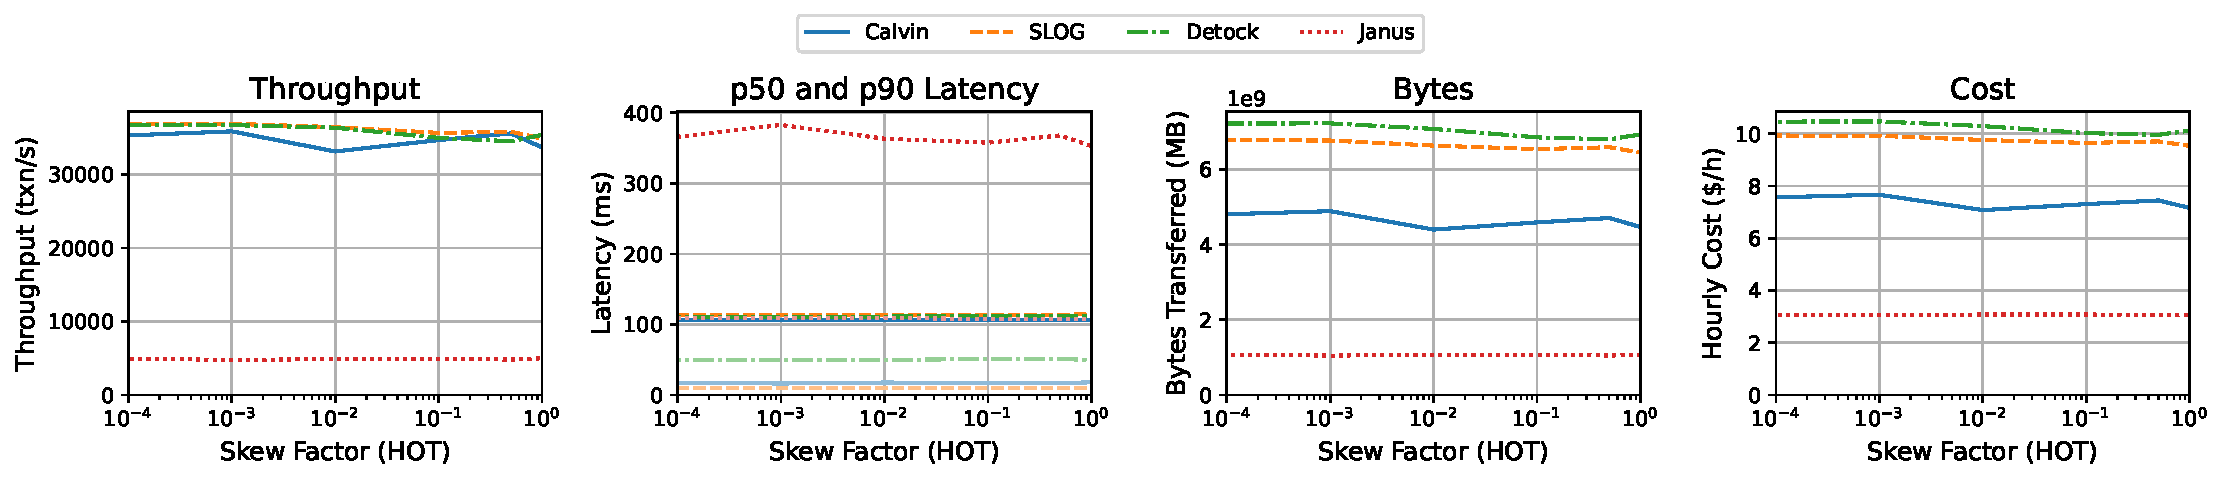
\includegraphics[width=1\textwidth]{figures/Skew.pdf}
    \caption{Skew Access Scenario Results.}
    \label{fig: skew-access-scenario}
\end{figure*}

\begin{figure*}[t]
    \centering
    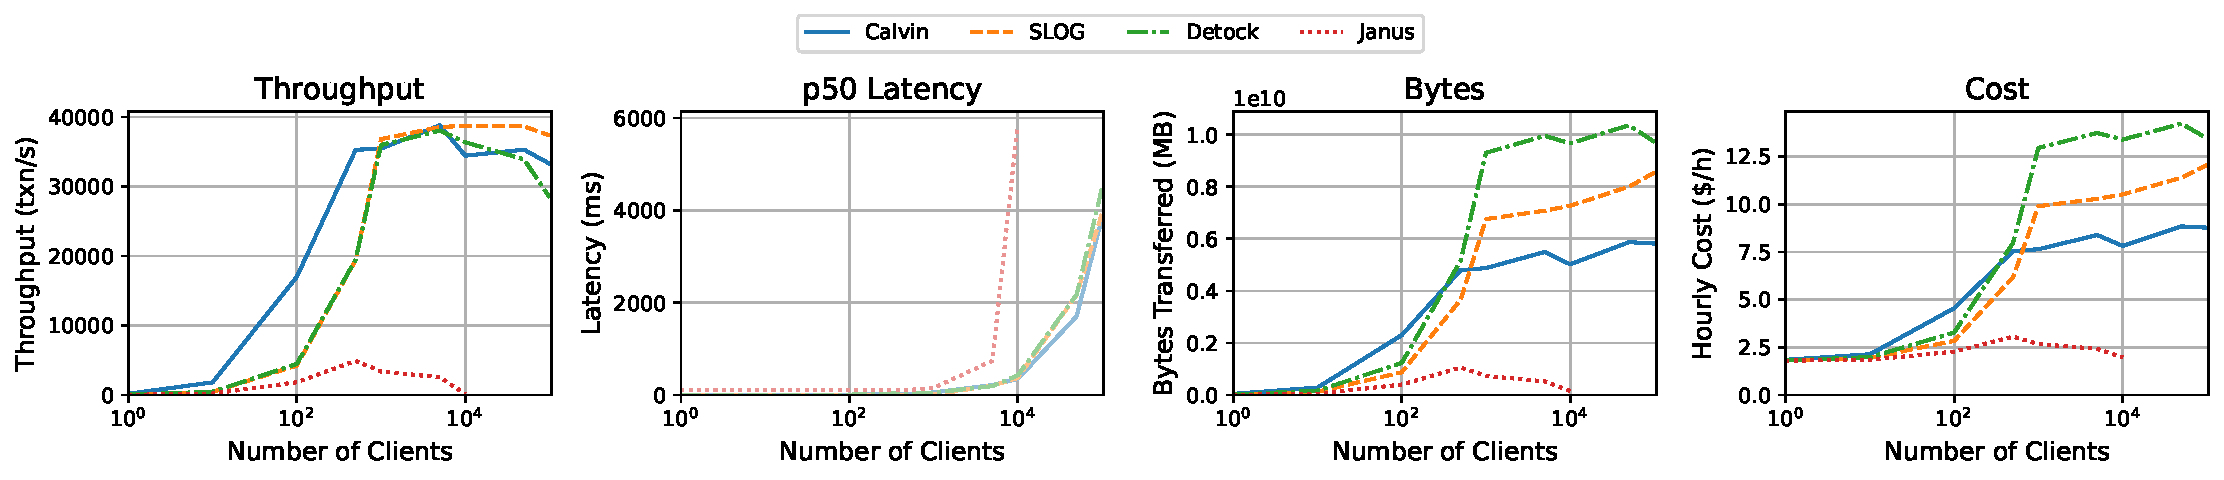
\includegraphics[width=1\textwidth]{figures/Scalability.pdf}
    \caption{Scalability Scenario Results.}
    \label{fig: scalability-access-scenario}
\end{figure*}

\section{Experimental Setup and Results}
\label{sec: experimental-setup-and-results}
This chapter presents our deployment setup, the methodology used for performance measurement, and the results obtained under a range of different experimental scenarios.

\subsection{Deployment and Metrics Collection}
\label{subsec: deployment-and-metrics-collection}
We conducted all experiments on a dedicated 4-node high-performance cluster located in our university. Each node is equipped with dual AMD EPYC 7H12 processors (resulting in 256 hardware threads) and 503 GiB of RAM. The nodes are interconnected via 10 Gigabit Ethernet.

In our experiments, we simulated a geo-distributed deployment by using all four physical nodes and injecting artificial network latency between them. Both clients and servers are deployed as Docker containers to ensure a clean and reproducible environment. The Figure~\ref{fig: overall-architecture} illustrates the setup. The data is divided into two partitions and fully replicated across two different regions. So, each region consists of two server containers that hold a complete copy of both partitions.  Unless stated otherwise, the clients are uniformly distributed across the two regions, and the number of client containers is varied between experiments to test scalability. By default, intra-region communication takes 0.5 ms round-trip time (RTT), while inter-region communication takes 50 ms.

For performance evaluation, each client container collects local metrics during execution, which are then aggregated by a centralized admin. The metrics we focus on are throughput, latency, abort rates, and bytes transferred, and we also estimate the operational cost. Throughput and abort rates are measured directly by the application logic, while latency and bytes transferred are collected using system-level network monitoring tools. Additionally, we estimate the cost by monitoring the resource utilization within the server containers and tracking the overall network usage.  

\begin{table}[htbp]
  \centering
  \begin{tabular*}{\linewidth}{@{\extracolsep{\fill}} l r r r r}
    \toprule
               & \textbf{A-P1} & \textbf{A-P2} & \textbf{B-P1} & \textbf{B-P2} \\ \midrule
    \textbf{A-P1} & —      & 0.15 ms & 100 ms & 100 ms \\
    \textbf{A-P2} & —      & —      & 100 ms & 100 ms \\
    \textbf{B-P1} & —      & —      & —      & 0.15 ms \\
    \textbf{B-P2} & —      & —      & —      & —      \\ \bottomrule
  \end{tabular*}
  \caption{Round-trip times (RTT) of all unordered pairs of machines. We uniquely identify the machines with the label \textit{Region-Partition} (e.g., \textit{A-P1} is the partition 1 from region A).}
  \label{tab: rtt-machines}
\end{table}

\subsection{Evaluation Scenarios and Results}
\label{subsec: evaluation-scenarios-and-results}
We now describe the experimental scenarios used in our evaluation. We designed these scenarios to systematically observe the impact of different system configurations on the transactional performance of the database systems. Each scenario is strongly connected with the tunable parameters shown in Figure~\ref{fig: overall-architecture}, which control the network conditions, the clients' placement, and the transactional load.

\subsubsection{Baseline Scenario}
\label{subsubsec: baseline-scenario}
In the baseline scenario, we aim to understand how each concurrency control protocol performs under standard conditions without artificial skew or complex network topologies. Namely, we vary only the fraction of \textit{multi-home transactions} among the \textit{OrderProduct} type while keeping the proportion of multi-partition transactions constant at 50\%. This scenario allows us to isolate the cost of coordination across different geographical regions.

Figure~\ref{fig: baseline-scenario} shows the metrics collected from each protocol. Among all systems, Janus performs significantly worse across all metrics, and the throughput is constant. This is primarily because Janus does not have the notion of multi-home transactions, and requires cross-region coordination even for transactions that could be executed locally. Therefore, Janus needs at least one WAN round-trip to commit, and when conflicts occur, it needs an additional round-trip.

Calvin also does not have the notion of multi-home transactions, but has a different behavior. It performs worse than SLOG and Detock when the proportion of multi-home transactions is low, but it stays constant, and it succeeds in overtaking them as the proportion increases. This is because Calvin relies on a deterministic global sequencer that orders all transactions. When most transactions are local, Calvin's overhead for global ordering becomes unnecessary and costly, but as the proportion of multi-home transactions increases, Calvin's global sequencer can coordinate them efficiently and get a better performance than SLOG and Detock, which incur a significant cost of handling multi-home transactions.  

\subsubsection{Skewed Access Scenario}
In the skewed access pattern, we study how each protocol handles the contention caused by an uneven access pattern. We fix the workload composition so that half of the \textit{OrderProduct} transactions are multi-home, and similarly, half of them are multi-partition. To introduce skew, we use the NURand distribution to define so-called \textit{hot records} that will be accessed more often depending on the \textit{skew factor} \cite{council2010tpc}.

As shown in Figure~\ref{fig: skew-access-scenario}, Detock and SLOG experience the most significant drop in throughput when increasing the skew factor from $0.001$ to $0.01$, after which their throughput stays approximately constant. This can be because both systems don't globally order single-home transactions, and thus, high contention can lead to higher aborts of the dependent transactions and local communication overhead between the partitions. In contrast, Calvin manages to have a more stable performance under skew thanks to the centralized sequencer. Janus, although not globally ordering the transactions, does not show a sensitivity to contention, which can indicate that contention is not the main bottleneck given the considered configurations. 

\subsubsection{Sunflower Topology Scenario}
TODO

\subsubsection{Scalability Scenario}
The scalability scenario focuses on evaluating how each protocol performs as we increase the number of clients, while keeping the workload composition fixed with half of the \textit{OrderProduct} transactions multi-home, and similarly, half of them multi-partition, and no added skew. We observe in Figure~\ref{fig: scalability-access-scenario} how SLOG, Detock, and Calvin all show similar improvements in throughput as the load increases, which demonstrates that these systems have good scalability given a balanced transactional workload. On the other hand, Janus scales even better than the other systems in the beginning, but quickly reaches a saturation point for $100$ clients, where the performance even starts to decrease.

\subsubsection{Network Delays Scenario}
TODO

\subsubsection{Packet Loss Scenario}
TODO





